\section{Zustandsraum-Darstellung}
Mit der ZRD können Systeme dargestellt werden. Im Gegensatz zur UTF sind ZRD numerisch stabilier und auch innere Systemkomponenten können damit dargestellt werden. ZRD können auch MIMO System darstellen.

\subsection{Definition}
\includegraphics[width=\columnwidth]{Images/zrd_übersicht}

\begin{align*}
	\dot{x}(t) &= \mathbf{A}x(t) + \mathbf{B}u(t) \qquad \text{(Zustandgleichung)} \\
	\dot{y}(t) &= \mathbf{C}x(t) + \mathbf{D}u(t) \qquad \text{(Ausgangsgleichung)}
\end{align*}

Die Matrizen sind folgendermassen definiert:\\
\begin{tabular}{ll}
	\textbf{A} & Systemmatrix $(n\times n)$ \\
	\textbf{B} & Steuer- oder Eingangsmatrix $(n \times m)$ \\
	\textbf{C} & Beobachtungs- oder Ausgangsmatrix $(k\times n)$ \\
	\textbf{D} & Übergangs- oder Durchgangsmatrix $(k\times m)$
\end{tabular}

Wobei \textbf{m} die Anzahl Eingänge, \textbf{n} Anzahl Integratoren (Ordnung) und \textbf{k} Anzahl Ausgänge.

\noindent Allgemeine SFD für 2.Ordnung
\begin{center}
	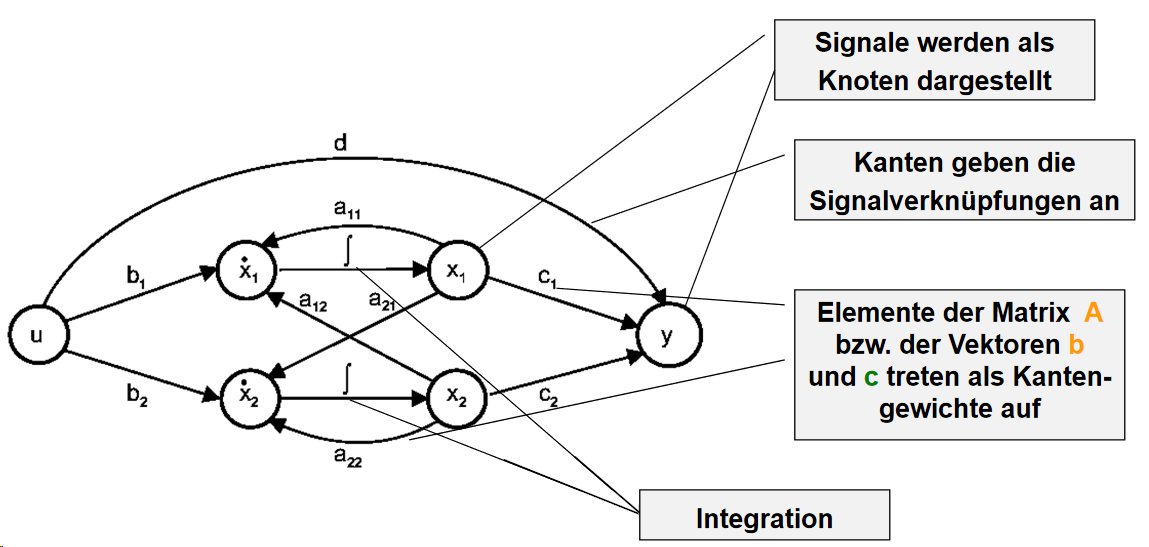
\includegraphics[width=\columnwidth]{Images/zrd}
\end{center}

\noindent\textbf{Beispiel Diagram}:
\begin{center}
	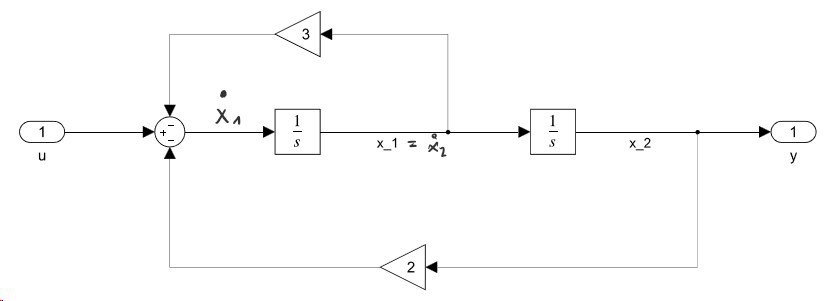
\includegraphics[width=\columnwidth]{Images/zrd1}
\end{center}
\begin{align*}
	\begin{pmatrix}	\dot{x}_1 & \dot{x}_2 \end{pmatrix} &=\overbrace{ \begin{pmatrix} -3 & -2 \\ 1 & 0 \end{pmatrix}}^{A}
	\begin{pmatrix}
		x_1 \\ x_2
	\end{pmatrix} + \overbrace{\begin{pmatrix}
			1 \\ 0
	\end{pmatrix}}^{B}u \\
	y &= \underbrace{\begin{pmatrix}
			0 & 1
	\end{pmatrix}}_{C} \begin{pmatrix}
x_1 \\ x_2
\end{pmatrix} + \underbrace{0}_{D}u
\end{align*}

\noindent\textbf{Beispiel DGL}:
\[
\dddot{y} + 8\ddot{y} + 21 \dot{y} + 18y = u
\]
Daraus lassen sich nun folgende DGL 1. Ordnung definieren $\begin{cases}\begin{matrix}
	x_1 = y \\
	x_2 = \dot{y}\\
	x_3 = \ddot{y}
\end{matrix}\end{cases}$. Anschliessend höchste Ableitung der ursprünglichen DGL Umformen und mit Zuständen ersetzen:
\begin{align*}
	\dot{x}_1 = \dot{y} &= x_2\\
	\dot{x}_2 = \ddot{y} &= x_3 \\
	\dot{x}_3 = \dddot{y} &= u - 8x_3 - 21x_2 -18x_1 \\
\end{align*}
Daraus lassen sich nun die ZRD Matrizen herleiten:
\begin{align*}
	\begin{pmatrix}
		\dot{x}_1 \\		\dot{x}_2 \\		\dot{x}_3 \\
	\end{pmatrix} &= \begin{pmatrix}
	0 & 1 & 0 \\
	0 &0 &1 \\
	-18 & -21 & -8
\end{pmatrix}\begin{pmatrix}
{x}_1 \\		{x}_2 \\		{x}_3 \\
\end{pmatrix} + \begin{pmatrix}
0 \\ 0 \\ 1
\end{pmatrix}u \\
y &= \begin{pmatrix}
	1 & 0 &0
\end{pmatrix}\begin{pmatrix}
{x}_1 \\		{x}_2 \\		{x}_3 \\
\end{pmatrix} + 0\cdot u
\end{align*}

Für ZRD von UTF siehe auch \script{267}. 


\subsection{Äquivalenz}
Um eine neue Zustandmatrix $\xi(t)$ zu erhalten, kann diese vom Ursprung Transformiert werden mit Transformationmatrix $T$.
\begin{align*}
	\dot{\xi}(t) &= \overbrace{\mathbf{TAT^{-1}}}^{\hat{A}} \xi(t) + \overbrace{\mathbf{TB}}^{\hat{B}} u(t)\\
	y(t) &= \overbrace{\mathbf{CT^{-1}}}^{\hat{C}}\xi(t) + \overbrace{\mathbf{D}}^{\hat{D}}u(t)
\end{align*}


\subsection{Übertragugnsfunktion}
Falls Anfangsbedingungen Null $x(0) = 0$ ist, folgt mit Einheitsmatrix $I$:
\[
\mathbf{H}(s) = \frac{Y(s)}{U(s)} = \mathbf{C}(s\mathbf{I} - \mathbf{A})^{-1}\mathbf{B} + \mathbf{D}
\]

\subsection{Fundamentalmatrix}
Die Fundamentalmatrix ist eine von $n$ linear unabhängige Lösungen einer homogenen Differentialgleichung $n$-ter Ordnung. Deren \textbf{Eigenschaften} sind:
\begin{itemize}[nosep]
	\item $\mathbf{\Phi}(0)  = \mathbf{I}$
	\item $\mathbf{\Phi}^{-1}(t) = \mathbf{\Phi}(-t)$, $\mathbf{\Phi}(t)$ ist immer invertierbar
	\item $\mathbf{\Phi}(t)^{k} = \mathbf{\Phi}(kt)$
	\item $\mathbf{\Phi}(t_1)\mathbf{\Phi}(t_2) = \mathbf{\Phi}(t_1 + t_2)$
	\item $\mathbf{\Phi}(t_2 - t_1)\mathbf{\Phi}(t_1 - t_0) = \mathbf{\Phi}(t_2 - t_0)$
\end{itemize}
~\\
Die \textbf{Impulsantwort} $h(t)$ eines SISO-Systems erhalten wir indem $h(t) = \mathbf{C}\mathbf{\Phi}(t)\mathbf{B} + \mathbf{D}\delta(t)$ rechnen.
~\\~\\
Um die Fundamentalmatrix $\mathbf{\Phi}(t)$ zu berechnen sind folgende Methoden möglich:


\textbf{Laplace-Transformation}
\[
\mathbf{\Phi}(t) = \mathcal{L}^{-1}\left\{(s\mathbf{I} - \mathbf{A})^{-1}\right\}
\]

\textbf{Diagonalisierung}
Dabei sind $\lambda_n$ die Eigenwerte von $\mathbf{A}$:
\[
\mathbf{\Phi}(t) = e^{\mathbf{A}\cdot t} = \mathbf{V}\begin{pmatrix}
	e^{\lambda_1t} & \dots & 0 \\
	\vdots & \ddots & \vdots \\
	0 & \dots & 	e^{\lambda_nt}
\end{pmatrix}\mathbf{V}^{-1}
\]

\subsubsection{Reihenentwicklung}
Substitution mit $\mathbf{A} = \begin{pmatrix}
	a & 0 \\ 1 & c
\end{pmatrix}$, damit lässt sich eine Summe von $\mathbf{A}^k$ berechnen:
\[
\mathbf{A}^k = \begin{pmatrix}
	a^k & 0 \\
	\sum\limits_{p = 0}^{k - 1}a^{k-p-1}c^p & c^k
\end{pmatrix}
\]

\textbf{Tip:} Folgender Ausdruck wird oft verwendet: $e^{\mathbf{A}t} = \sum\limits_{k=0}^{\infty}\frac{\mathbf{A}^kt^k}{k!}$

\subsection{Stabilität}
Die Eigenwerte von Systemmatrix $\mathbf{A}$ entsprechen den Polstellen des Systems. Ein LTI-System ist asymptotisch stabil, wenn alle Eigenwerte einen negativen Realanteil besitzen. Umgekehrt gilt diese Aussage nicht. In der \textbf{diagonalisierten Normalform} (Siehe dazu Kapitel \ref{diag}) können die Eigenwerte direkt ausgelesen werden.

\subsection{Normalformen}
Wenn ein System entweder als UTF oder DGL vorhanden ist, lässt sich eine Matrix direkt übertragen:
\[
H(s) = \frac{b_{m}s^{m} + \dots b_1s + b_0}{s^n + a_{n-1}s^{n-1} + \dots a_1s + a_0}
\]
oder \[
a_ny^{(n)}(t) + \dots + a_1\dot{y}(t) + a_0y(t) = b_mu^{(m)}(t) + \dots + b_1\dot{u}(t) + b_0u(t)
\]

\subsubsection{Regelungsnormalform}
\script{267}:
\begin{align*}
 \begin{pmatrix}  \dot{x}_1 \\ 	\dot{x}_2 \\ \vdots \\ \dot{x}_n \\ \end{pmatrix}
 &=
 \begin{pmatrix}
 	0 & 1 & 0 & \dots & 0\\
 	0 & 0 & 1 & \dots & 0\\
 	\vdots & \vdots & \vdots & \ddots & \vdots \\
 	-a_0 & -a_1 & -a_2 & \dots & -a_{n-1}
 \end{pmatrix}\cdot
\begin{pmatrix}  {x}_1 \\ 	{x}_2 \\ \vdots\\ {x}_n \\ \end{pmatrix} +
\begin{pmatrix}  0 \\ 0 \\ \vdots \\1 \\ \end{pmatrix}
\\
y(t) &= \begin{pmatrix}
	b_0-a_0b_n & b_1 - a_1b_n & \dots & b_{n-1}-a_{n-1}b_n
\end{pmatrix}\cdot
\begin{pmatrix}  {x}_1 \\ 	{x}_2 \\ \vdots\\ {x}_n \\ \end{pmatrix}
+ {b_n}\cdot u(t)
\end{align*}
Weil $m<n$ meist ist, vereinfacht sich $b_n = 0$

\subsubsection{Diagonalform}\label{diag}
Diese Form eignet sich besonders um die Stabilität eines Systems zu beurteilen.
\todo{}
Die Polstellen der UTF (Tip: Partialbruchzerlegung) entsprechen den Eigenwerten des Systems, welche auf der Diagonalmatrix liegen.

\subsubsection{Beobachtbarkeit}
Eine \textbf{beobachtbares} System heisst dabei, dass sich ein Zustand $x$ durch messen des Ausgangssignal $y$ bestimmen lässt. Die Form ist dual zur Reglungsnormalform \script{277}.
\begin{align*}
	\begin{pmatrix}  \dot{x}_1 \\ 	\dot{x}_2 \\ \vdots \\ \dot{x}_n \\ \end{pmatrix}
	&=
	\begin{pmatrix}
		0 & 0 & 0 & \dots & -a_0\\
		1 & 0 & 0 & \dots & -a_1\\
		\vdots & \vdots & \vdots & \ddots & \vdots \\
		0 & 0 & 1 & \dots & -a_{n-1}
	\end{pmatrix}\cdot
	\begin{pmatrix}  {x}_1 \\ 	{x}_2 \\ \vdots\\ {x}_n \\ \end{pmatrix} +
	\begin{pmatrix} b_0-a_0b_n \\ b_1 - a_1b_n \\ \dots \\ b_{n-1}-a_{n-1}b_n\end{pmatrix}
	\\
	y(t) &= \begin{pmatrix}
		 0 & 0 & \dots &1 \\ 
	\end{pmatrix}\cdot
	\begin{pmatrix}  {x}_1 \\ 	{x}_2 \\ \vdots\\ {x}_n \\ \end{pmatrix}
	+ {b_n}\cdot u(t)
\end{align*}

Mit $\det(\mathbf{Q}_B) \neq 0$ lässt sich bestimmen, ob ein System beobachtbar ist.
\[
\mathbf{Q}_B = \begin{pmatrix}
	\mathbf{C} \\
	\mathbf{CA} \\
	\mathbf{CA^2} \\
	\vdots\\
	\mathbf{CA^{n-1}} \\
\end{pmatrix}
\]
In der Diagonalisierten Form, darf die Matrix $\mathbf{C}$ keine $0$ Einträge beinhalten.

\subsubsection{Steuerbarkeit}
Die Steuerbarkeit beschreibt, wie der Zustand $x$ durch den Eingang $u$ beeinflusst werden kann.
Mit $\det(\mathbf{Q}_S) \neq 0$ lässt sich bestimmen, ob ein System beobachtbar ist.
\[
\mathbf{Q}_S = \begin{pmatrix}
	\mathbf{B} &
	\mathbf{AB} &
	\mathbf{A^2B} &
	\dots&
	\mathbf{A^{n-1}B} 
\end{pmatrix}
\]
In der Diagonalisierten Form, darf die Matrix $\mathbf{B}$ keine $0$ Einträge beinhalten.
